
\chapter{Introduzione}
L'obiettivo del progetto realizzato è quello di integrare la libreria OROCOS KDL (\url{https://www.orocos.org/kdl.html}) nel component framework \textit{STAR} per definire un'applicazione che consente di inviare al robot comandi di posizione della pinza montata all'estremità del robot manipolatore P-Rob 3 (\Fig\ref{fig:prob3}) rispetto al sistema di riferimento cartesiano alla base del robot.
\begin{figure}[b!]
	\centering
	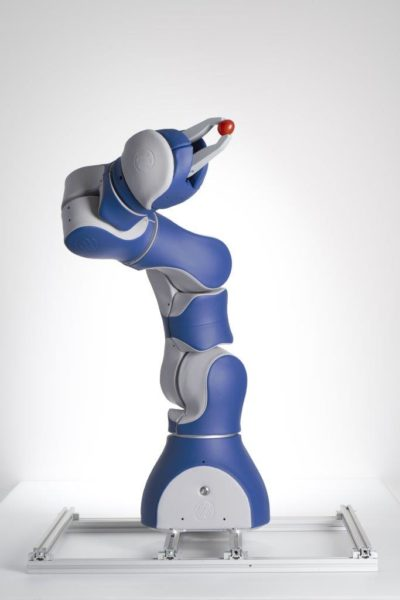
\includegraphics[width=0.4\linewidth]{./ImageFiles/P-Rob 3.jpg}
	\caption{Robot manipolatore P-Rob 3.}
	\label{fig:prob3}
\end{figure}
In particolare, si sono sviluppate le seguenti funzionalità:
\begin{itemize}
	\item calcolo della posizione della pinza rispetto al sistema di riferimento alla base del robot a partire dal valore degli angoli dei giunti (cinematica diretta);
	\item calcolo del valore dei giunti a partire dalla posizione della pinza rispetto al sistema di riferimento alla base del robot (cinematica inversa);
	\item calcolo di un percorso lineare a partire da una posizione iniziale e una finale della pinza.
\end{itemize}

\chapter{Libreria OROCOS KDL}
\section{Installazione}
Per effettuare i calcoli cinematici si è scelto di utilizzare la libreria OROCOS KDL, che implementa le funzionalità base come il calcolo della cinematica diretta e inversa per un robot. Seguendo la guida di installazione disponibile nella documentazione (\url{https://www.orocos.org/wiki/Installation_Manual.html}), la libreria è stata installata nel framework \textit{STAR} al seguente percorso: STAR/AutonomousRobot/Libraries/others/orocos\_kinematics\_dynamics. Inoltre, per semplificare alcune operazioni di inizializzazione della libreria KDL, è stato installata la libreria \textit{kdl parser} nella cartella STAR/AutonomousRobot/Libraries/others/kdl\_parser, seguendo le istruzioni di installazione reperibili al seguente link \url{STAR/AutonomousRobot/Libraries/others/orocos\_kinematics\_dynamics}. Infine, è stato modificato il file \textit{ev-star.sh} inserendo le informazioni per includere i file e recuperare i binari delle librerie installate quando vengono compilati componenti e plugin.

\section{Definizione del modello del robot}
La libreria KDL ha bisogno di conoscere la struttura cinematica del robot. La catena cinematica del robot è stata definita in un file .urdf (\url{http://wiki.ros.org/urdf}), nel quale sono descritti in modo standard tutti i parametri, quali ad esempio il numero, la tipologia e i limiti dei giunti e la lunghezza dei link. Per definire questo file, si è partiti dal modello fornito sulla pagina github del produttore (\url{https://github.com/fp-robotics/fp_descriptions}), generando il file urdf seguendo la procedura indicata. Successivamente, il file è stato modificato per estrapolare le informazioni rilevanti per il progetto e, eseguendo delle prove con l'interfaccia web fornita dal produttore del robot, sono stati verificati alcuni dati presenti nell'urdf. La catena cinematica descritta dall'urdf è riportata in figura \ref{fig:urdf_prob3}.

\newpage
\begin{figure}[tbh]
	\centering
	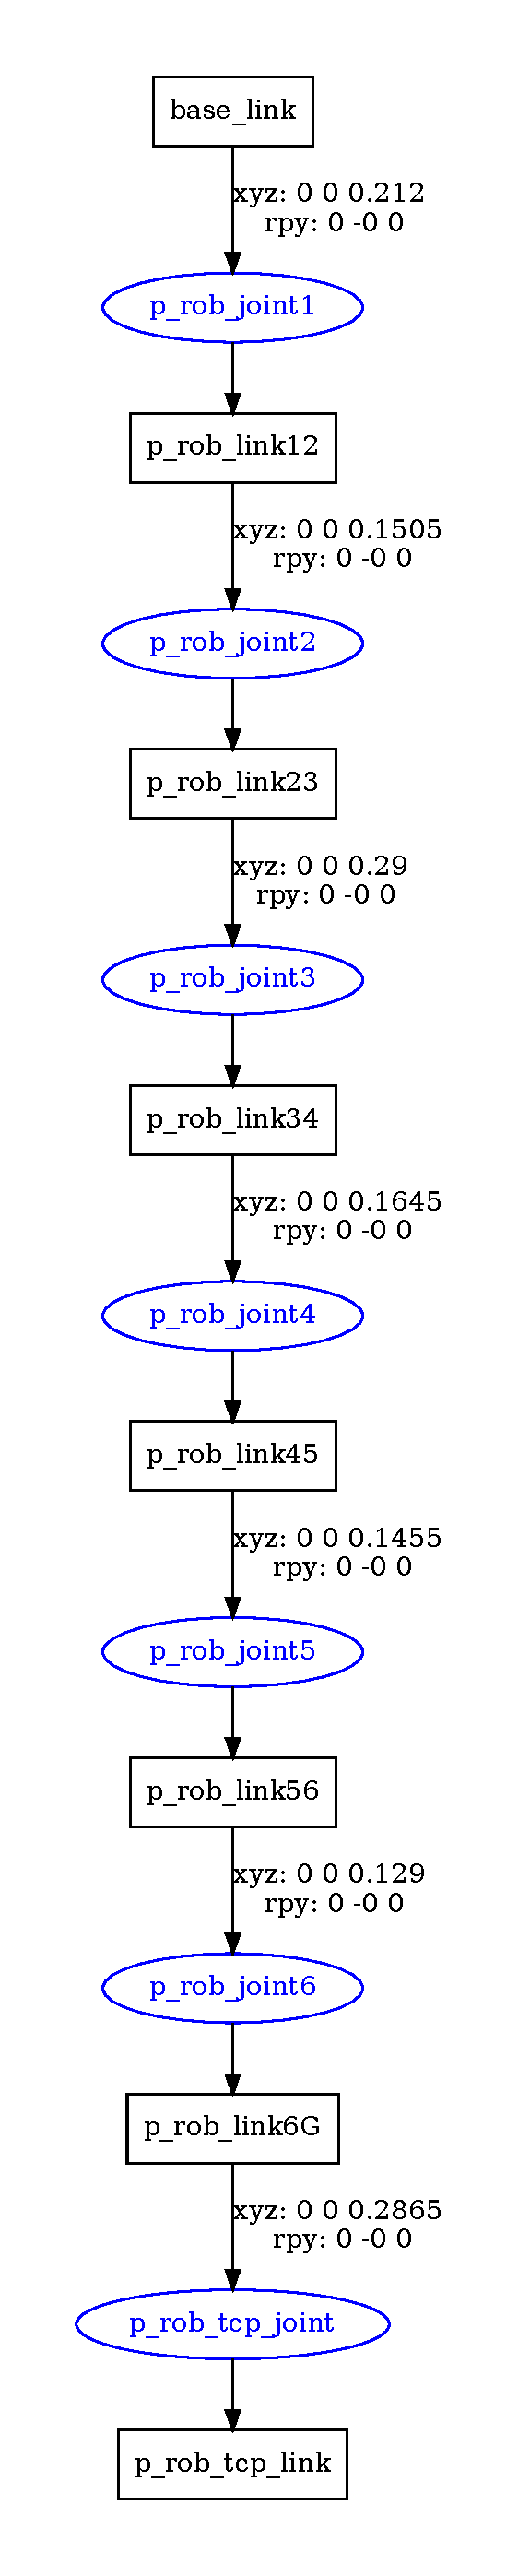
\includegraphics[width=0.3\linewidth]{./OtherFiles/p_rob.pdf}
	\caption{Catena cinematica descritta dal file urdf.}
	\label{fig:urdf_prob3}
\end{figure}

Nel file urdf, che è strutturato come un file xml, è possibile specificare i giunti e i link del robot tramite i seguenti elementi:
\begin{itemize}
	\item \tl link name="xxx"\tr...\tl /link\tr, che descrive un link;
	\item \tl joint name="yyy" type="zzz"\tr...\tl /joint\tr, che descrive un giunto; il robot utilizzato è costituito da sei giunti di rotazione, per cui il tipo dei giunti è definito come "revolute".
\end{itemize}
All'interno degli elementi è possibile poi specificare diverse caratteristiche tra le quali (elenco completo reperibile al link \url{http://wiki.ros.org/urdf/XML/joint}):
\begin{itemize}
	\item  \tl parent link="xxx"/\tr\ e \tl child link="yyy"/\tr\ indicano rispettivamente il link padre e il link figlio di un giunto;
	\item \tl axis xyz="0 1 0"/\tr\ indica l'asse di rotazione del giunto;
	\item  \tl origin xyz="0 0 0.29"/\tr\ indica la rototraslazione tra il link padre e il link figlio.
\end{itemize}
Per descrivere il robot utilizzato, sono quindi stati definiti sei giunti di rotazione (tre con asse di rotazione lungo l'asse z e tre con asse di rotazione lungo l'asse y) e sette link dalla base del robot fino al centro di presa. Sono stati poi aggiunti un giunto di tipo \textit{fisso} e un link terminale per rappresentare correttamente il centro di presa.

\clearpage

\section{KDL Paser}

\todo{desrivere il metodo loadChainFromUrdf per inizializzare la libreria}

\section{Sistemi di riferimento del robot}

Nelle figure \ref{fig:base_frame} e \ref{fig:tool_frame} sono riportati i sistemi di riferimento rispetto alla base del robot e del tool che sono stati considerati nel progetto.

\begin{figure}[tbh]
	\centering
	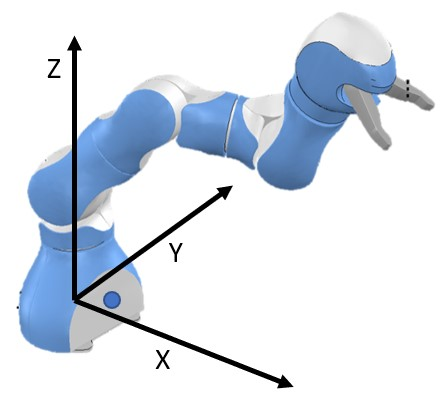
\includegraphics[width=0.5\linewidth]{./ImageFiles/prob_frame_base}
	\caption{Sistema di riferimento alla base del robot.}
	\label{fig:base_frame}
\end{figure}

\begin{figure}[tbh]
	\centering
	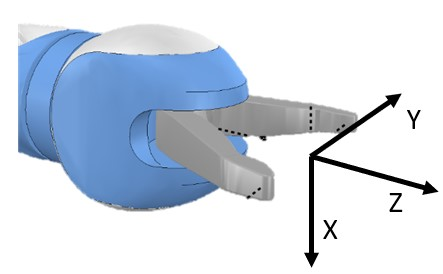
\includegraphics[width=0.5\linewidth]{./ImageFiles/prob_frame_tool.jpg}
	\caption{Sistema di riferimento del tool.}
	\label{fig:tool_frame}
\end{figure}

\section{Cinematica diretta e inversa}
\section{Traiettoria lineare}
\todo{Descriviamo magari qui il funzionamento base delle funzioni e poi facciamo una sezione con invece la definizione di come sono stati introdotti in star quindi plugin e componenti?}

\chapter{Implementazione in star} \todo{nome solo per far capire la sezione (es diagramma componeti)}
\section{Plugin: PluginArmPRob3Kinematics}
\section{Componente: ArmDriver e ToolInput}
